\documentclass[11pt,spanish]{article}

\usepackage[utf8]{inputenc} % Required for inputting international characters
\usepackage[T1]{fontenc}
\usepackage{mathpazo} % Palatino font
\usepackage{amsmath}
\usepackage{selinput}
\SelectInputMappings{%
  aacute={á},
  ntilde={ñ},
  Euro={€}
}
\usepackage{babel}
\usepackage{hyperref}
\usepackage{multirow}
\usepackage{caption}
\usepackage{graphicx}

\hypersetup{
    colorlinks,
    citecolor=black,
    filecolor=black,
    linkcolor=black,
    urlcolor=blue
}
\begin{document}
%------------------------------------------------------------------------------------------

	%---------------------------%
	%	Stop Numbering Pages	%
	%---------------------------%

	\pagenumbering{gobble}

%------------------------------------------------------------------------------------------
	\begin{titlepage} % Suppresses displaying the page number on the title page and the subsequent page counts as page 1
	
	\newcommand{\HRule}{\rule{\linewidth}{0.5mm}} % Defines a new command for horizontal lines, change thickness here
	
	\center % Centre everything on the page
	
	%---------------%
	%	Encabezados	%
	%---------------%
	
	\textsc{\LARGE Universidad Carlos III de Madrid}\\[1.5cm] % Main heading such as the name of your university/college
	
	\textsc{\Large Grado en Ingeniería Informática}\\[0.5cm] % Major heading such as course name
	
	\textsc{\large Heurística y Optimización}\\[0.5cm] % Minor heading such as course title
	
	%-----------%
	%	Titulo	%
	%-----------%
	
	\HRule\\[0.4cm]
	
	{\huge\bfseries Práctica: Programación Lineal}\\[0.4cm] % Title of your document
	
	\HRule\\[1.5cm]
	
	%---------------%
	%	Author(s)	%
	%---------------%
	
	\begin{minipage}{0.7\textwidth}
		\begin{flushleft}
			\large
			\textit{Autores}\\
			\textsc{Alberto Villanueva Nieto\ \ \ \ 100374691}\\
            \textsc{Cristian Cabrera Pinto\ \ \ \ \ \ \ \ \ \ 100363778}
		\end{flushleft}
	\end{minipage}

	%-----------%
	%	Date	%
	%-----------%
	
	\vfill\vfill\vfill % Position the date 3/4 down the remaining page
	
	{\large\today} % Date, change the \today to a set date if you want to be precise
	
	\vfill % Push the date up 1/4 of the remaining page
	
	\end{titlepage}
	\newpage
%------------------------------------------------------------------------------------------
	\tableofcontents
	\newpage
%------------------------------------------------------------------------------------------

	%---------------------------%
	%	Start Numbering Pages	%
	%---------------------------%

	\pagenumbering{arabic}

%------------------------------------------------------------------------------------------
	\section{Intorducción}
	En este documento se explican los modelos de los ejercicios de programación lineal y dinámica, en los de lineal explicando que representa cada conjunto, variable, y restricción. A continuación se analizan los resultados de los modelos, su complejidad y las ventajas y desventajas de usar calc repecto a GLPK y finalmente se procede a la conclusión de la práctica.

	\section{Descripción de los modelos}
		\subsection{Modelo para la compra}
			En esta parte se pide minimizar el coste de la compra de unos elementos entre 2 fábricas en función de sus límites de inventario donde el precio del elemento y del transporte desde la fábrica hasta donde se quieren tener varia en función de la fábrica.
			\subsubsection{Conjuntos}
			Para poder expresar las variables, los parámetros y las ecuaciones de una forma más descriptiva se va a hacer uso de un conjunto que describe los distintos tipos de productos que hay:
			$$ productos := \{loc, vag1, vag2, cont20, cont40\} $$
			\subsubsection{Variables de decisión}
			Aunque a primera vista puede parecer que se necesitan 10 variables de decisión (por cada tipo de elemento en cada fábrica) sin embargo, si se sabe los elementos totales que se quieren obtener y los que se van a comprar en una de las dos fábricas, los elementos que se compran en la fábrica restante es la diferencia entre los elementos que se quieren obtener y los que se compran en la primera fábrica, de este modo nuestras variables de decisión serían:
			\begin{align*}
			x_{loc}:& Locomotoras\ compradas\ en\ la\ primera\ f\acute{a}brica \\
			x_{vag1}:& Vagones\ de\ tipo\ 1\ comprados\ en\ la\ primera\ f\acute{a}brica \\
			x_{vag2}:& Vagones\ de\ tipo\ 2\ comprados\ en\ la\ primera\ f\acute{a}brica \\
			x_{cont20}:& Contenedroes\ de\ 20'\ comprados\ en\ la\ primera\ f\acute{a}brica \\
			x_{cont40}:& Contenedroes\ de\ 40'\ comprados\ en\ la\ primera\ f\acute{a}brica 
			\end{align*}
			
			\subsubsection{Parámetros}
			Para el cálculo de la función objetivo y de las restricciones se han hecho con respecto a los datos que se nos proporcionaban en el enunciado:
			
			\begin{align*}
			Necesidad_p:& Cantidad\ de\ productos\ tipo\ p\ que\ se\ necesitan. \\
			Stock\ Primera_p:& Cantidad\ de\ productos\ tipo\ p\ que\ la\ primera\ f\acute{a}brica\ puede\ proveer. \\
			Stock\ Segunda_p:& Cantidad\ de\ productos\ tipo\ p\ que\ la\ segunda\ f\acute{a}brica\ puede\ proveer. \\
			Coste\ Primera_p:& Coste\ de\ comprar\ y\ transportar\ un\ elemento\ p\ de\ la\ primera f\acute{a}brica\ al\ destino. \\
			Coste\ Segunda_p:& Coste\ de\ comprar\ y\ transportar\ un\ elemento\ p\ de\ la\ segunda f\acute{a}brica\ al\ destino. \\
			&\forall p \in productos 
			\end{align*}
			\captionof{table}{Parámetros de compra}
			\label{tab:params1}
			\begin{tabular}{ |c||c|c|c|c|c|  }	
			 	\hline
			 	\multirow{2}{*}{Parámetro} & \multirow{2}{*}{Locomotoras} &  \multicolumn{2}{|c|}{Vagones} & \multicolumn{2}{|c|}{Contenedores} \\
			 	& & Tipo 1 & Tipo 2 & 20' & 40'\\
			 	\hline
			 	Necesidad & 3 & 3 & 2 & 4 & 4 \\
			 	Stock Primera & 2 & 3 & 2 & 4 & 4 \\
			 	Stock Segunda & 3 & 3 & 2 & 2 & 3 \\
 			 	Coste Primera & 100200 & 10500 & 20040 & 20080 & 30040 \\
			 	Coste Segunda & 200220 & 3440 & 5660 & 25220 & 40220 \\
				\hline
			\end{tabular}

			\subsubsection{Función objetivo}
			Para la función objetivo se pretende minimizar el coste de comprar los productos en ambas fábricas:
			$$
			minimizar\ coste = \sum_p^{productos} (x_p * Coste Primera_p + (Necesidad_p - x_p) * Coste Segunda_p)
			$$
			\subsubsection{Restricciones}
			El problema de optimización esta restringido con que las variables sean no negativas (\ref{eq:numeroNoNegativo}) enteras (\ref{eq:numeroEntero}), que se compren más productos en la primera fábrica que en la segunda (\ref{eq:prioridadTiempo}), que el precio gastado en cada fábrica no supere en un 10\% al gastado en al otra (\ref{eq:monopolio_1a})(\ref{eq:monopolio_2a}) y que los productos que se compren en cada una de las fábricas esten dentro del límite que tenga esa fábrica (\ref{eq:SeCumpleStockPrimera})(\ref{eq:SeCumpleStockSegunda}).
			\begin{equation}
				\label{eq:numeroNoNegativo}
				x_p \geq 0, \forall p \in productos
			\end{equation}
			\begin{equation}
				\label{eq:numeroEntero}
				x_p \in \mathbb{Z} , \forall p \in productos
			\end{equation}
			\begin{equation}
				\label{eq:prioridadTiempo}
				-1 + \sum_p^{productos} x_p > \sum_p^productos (Necesidad_p - x_p)
			\end{equation}
			\begin{equation}
				\label{eq:monopolio_1a}
				1.1*\sum_p^{productos} x_p*CostePrimera_p \geq \sum_p^{productos} (Necesidad_p - x_p)*CosteSegunda_p
			\end{equation}
			\begin{equation}
				\label{eq:monopolio_2a}
				\sum_p^{productos} x_p*CostePrimera_p \leq 1.1*\sum_p^{productos} (Necesidad_p - x_p)*CosteSegunda_p
			\end{equation}
			\begin{equation}
				\label{eq:SeCumpleStockPrimera}
				x_p \leq StockPrimera_p, \forall p \in productos
			\end{equation}
			\begin{equation}
				\label{eq:SeCumpleStockSegunda}
				Necesidad - x_p \leq StockSegunda_p, \forall p \in productos
			\end{equation}
		\subsection{Modelo para la asignación}
		En esta parte se pide minimizar el coste del transporte de una cantidad de toneladas en 2 rutas, para ello se dispone de los elementos que se han comprado en la parte anterior donde los contenedores y vagones tienen un límite dado por su tipo.
			\subsubsection{Conjuntos}
			Para expresar las variables de decisión y los parámetros con respecto a los elementos en especifico creamos varios conjuntos para asi poder tener bien controlado a que parámetro se hace referencia:
			\begin{align*}
				contenedores\ tipos :=& \{ Cont20, Cont40 \} \\
				contenedores_{Cont20} :=& \{ C1, C2, C3, C4 \} \\
				contenedores_{Cont40} :=& \{ C5, C6, C7, C8 \} \\
				contenedores todos :=& \bigcup_{ct}^{contenedores\ tipos} contenedores_{ct} \\
				vagones\ tipos :=& \{ Vag1, Vag2 \} \\
				vagones_{Vag1} :=& \{ V1, V2, V3 \} \\
				vagones_{Vag2} :=& \{ V4, V5 \} \\
				vagones todos :=& \bigcup_{vt}^{vagones\ tipos} vagones_{vt} \\
				locomotoras :=& \{ L1, L2, L3 \} \\
				rutas :=& \{ Madrid-Valencia, Madric-C\acute{a}diz \}
			\end{align*}
			\subsubsection{Variables de decisión}
			Al tratarse de un ejercicio de programación lineal de asignación, las variables son matrices binarias que representan la distribución de los elementos de las filas entre los elementos de las columnas. Por los requisitos que pide el enunciado las matrices que se necesitan son las siguientes:
			\begin{align*}
				CV_{contenedores\ todos\ x\ vagones\ todos} :& Indica\ en\ que\ vag\acute{o}n\ va\ cada\ contenedor.\text{\footnotemark} \\
				CR_{contenedores\ todos\ x\ rutas} :& Indica\ en\ que\ ruta\ va\ cada\ contenedor.\\
				VR_{vagones\ todos\ x\ rutas} :& Indica\ en\ que\ ruta\ va\ cada\ vag\acute{o}n.\\
				LR_{locomotoras\ x\ rutas} :& Indica\ en\ que\ ruta\ va\ cada\ locomotora.^1
			\end{align*}
			\footnotetext{Estas variables solo son necesarias porque el enunciado dice que se tienen que tener bien controladas donde va cada elemento, pero realmente si conoces que contenedores y que vagones van en una ruta, asignar los contenedores a los vagones es una tarea elemental, y con respecto a las locomotoras es aun más elemental ya que no hay restricciones en el enunciado luego se puede asumir que con una locomotora por ruta es suficiente.}

			\subsubsection{Parámetros}
			Para el cálculo de la función objetivo y las restricciones, se han sintetizado los datos del enunciado en los siguientes parámetros:
			\begin{align*}
				Distancia_r:& Distancia\ que\ tiene\ que\ recorrer\ un\ elemento\ en\ la\ ruta\ r.\\
				&\forall r \in rutas\\
				Mercancias_r:& Cantidad\ de\ mercancias\ que\ tiene\ que\ se\ tienen\ que\ trasladar\ en\ la\ ruta\ r.\\
				&\forall r \in rutas\\
				Traslado_{ct,r}:& Lo\ que\ cuesta\ trasladar\ un\ contenedor\ de\ tipo\ ct\ en\ la\ ruta\ r.\\
				&\forall ct \in contenedores\ tipos, \forall r \in rutas \\
				L\acute{i}mite\ Contenedor_{ct}:& La\ cantidad\ de\ mercancia\ que\ puede\ trasladar\ un\ contenedor\ de\ tipo\ ct.\\
				&\forall ct \in contenedores\ tipos\\
				L\acute{i}mite\ Vag\acute{o}n_{vt,ct}:& La\ cantidad\ de\ contenedores\ tipo\ ct\ que\ puede\ trasladar\ un\ vag\acute{o}n\ tipo\ vt.\\
				&\forall vt \in vagones\ todos, \forall ct \in contenedores\ tipos\\
			\end{align*}
			\\
			\captionof{table}{Parámetros de asignación. Rutas}
			\label{tab:params2rut}
			\begin{tabular}{ |c|c||c|c|  }
				\hline
				\multicolumn{2}{|c||}{}& Madrid-Valencia & Madrid-Cadiz \\
				\hline
				\multicolumn{2}{|c||}{Distancia} & 360 & 650\\
				\multicolumn{2}{|c||}{Mercancias} & 90 & 150\\
				\multirow{2}{*}{Traslado} & Cont20 & 10 & 20\\
				& Cont40 & 15 & 30\\
				\hline
			\end{tabular}
			\\
			\\
			\captionof{table}{Parámetros de asignación. Contenedores}
			\label{tab:params2cont}
			\begin{tabular}{ |c|c||c|c|  }
				\hline
				\multicolumn{2}{|c||}{}& Cont20 & Cont40 \\
				\hline
				\multicolumn{2}{|c||}{Límite Contenedor} & 32 & 67\\
				\multirow{2}{*}{Límite Vagón} & Vag1 & 2 & 0\\
				& Vag2 & 2 & 1\\
				\hline
			\end{tabular}

			\subsubsection{Función objetivo}
			Para la función objetivo se pretende minimizar el coste de trasladar los contenedores en las rutas.
			$$
			minimizar\ coste = \sum_r^{rutas} \left( \sum_{ct}^{contenedores\ tipos} \left( \sum_c^{contenedores_{ct}} CR_{c,r} \right) * Traslado_{ct,r} \right) * Distancia_r
			$$
			\subsubsection{Restricciones}
			El problema, por como esta presentado, presenta 3 restricciones muy claras; que se tienen que transportar cierta cantidad de mercancias en cada ruta (\ref{eq:SatisfaceMercancias}), que las rutas cumplan los límites de contenedores que los vagones asignados a esa ruta le permitan(\ref{eq:RutaCumpleLimitesContenedores}) y que se tiene que evitar el uso innecesario de vagones(\ref{eq:EvitaUsoInnecesario}). También, al tratarse de un problema de asignación, en nuestras variables, un elemento solo puede ser asignado a una cosa (\ref{eq:unaRutaPorContenedor}-\ref{eq:unVagonPorContenedor}) y además se asume tiene que haber al menos una locomotora en cada ruta (\ref{eq:alMenosUnaLocomotoraPorRuta}).\\
			Para asegurarse de que la coherencia entre las variables CV, VR, y VR se restringe que los vagones cumplan los límites de contenedores que pueden trasladar (\ref{eq:VagonesCumplenLimitesContenedores}), que se asignen a vagones los mismos contenedores que se asignan a rutas (\ref{eq:CoherenciaTotalidadContenedores}) y que, teniendo en cuenta esas otras dos restricciones, si un contenedor esta asignado a una vagón y un vagón esta asignado a una ruta, que el contenedor este asignado a esa ruta (\ref{eq:Coherencia_CV_CR}).\footnote{La forma más directa de hacer esto es usar un and, sin embargo trasladar un and del mundo binario al entero lo convierte en una multiplicación de variables por lo que deja de ser lineal, para solucionarlo se ha hecho una restricción (\ref{eq:Coherencia_CV_CR}) que te garantiza: a = 1 and b = 1 --> c = 1, pero si a o b es 0 no te garantiza que c sea 0, para completar esto y que así tenga la funcionalidad de una and se han usado otras 2 restricciones(\ref{eq:VagonesCumplenLimitesContenedores})(\ref{eq:CoherenciaTotalidadContenedores}).}
			$$
				CV_{c,v},CR_{c,r},VR_{v,r},LR_{l,r} \in \mathbb{Z}_2
			$$
			\begin{equation}
				\forall c \in contenedores\ todos, \forall v \in vagones\ todos, \forall l \in locomotoras, \forall r \in rutas	
			\end{equation}
			$$
				\sum_{ct}^{contenedores\ tipos}\left(\left( \sum_c^{contenedores{ct}} CR_{c,r} \right) * L\acute{i}mite\ Contenedor_{ct} \right) \geq  Mercancias_r;
			$$
			\begin{equation}
				\label{eq:SatisfaceMercancias}
				\forall r \in rutas
			\end{equation}
			$$
				\sum_c^{contenedores_{ct}} CR_{c,r} \leq \sum_{vt}^{vagones\ tipos} \left( \left(\sum_v^{vagones_{vt}}VR_{v,r}\right)*L\acute{i}mite\ Vag\acute{o}n_{vt,ct} \right);
			$$
			\begin{equation}
				\label{eq:RutaCumpleLimitesContenedores}
				\forall r \in rutas,\forall ct \in contenedores\ tipos
			\end{equation}
			
			\begin{equation}
				\label{eq:EvitaUsoInnecesario}
				-1+\sum_c^{contenedores\ todos} CR_{c,r} \geq \sum_v^{vagones\ todos} VR_{v,r};\ \forall r \in rutas
			\end{equation}
			$$
			\sum_c^{contenedores_{ct}}CV_{c,v} \leq L\acute{i}mite\ Vag\acute{o}n_{vt,ct};
			$$
			\begin{equation}
				\label{eq:VagonesCumplenLimitesContenedores}
				\ \forall vt \in vagones\ tipos, \forall v \in vagones_{vt}, \forall ct \in contenedores\ tipos
			\end{equation}
			\begin{equation}
				\label{eq:CoherenciaTotalidadContenedores}
				\sum_r^{rutas} CR_{c,r} = \sum_v^{vagones\ todos} CV_{c,v};\ \forall c \in contenedores\ todos
			\end{equation}
			\begin{equation}
				\label{eq:Coherencia_CV_CR}
				CR_{c,r}+CV_{c,v}-1<=VR_{v,r};\ \forall r \in rutas, \forall c \in contenedores\ todos, \forall v \in vagones\ todos
			\end{equation}


			\begin{equation}
				\label{eq:alMenosUnaLocomotoraPorRuta}
				\sum_l^{locomotoras}LR_{l,r} \geq 1;\ \forall r \in rutas
			\end{equation}
			\begin{equation}
				\label{eq:unaRutaPorContenedor}
				\sum_r^{rutas}CR_{c,r} \leq 1;\ \forall c \in contenedores\ todos
			\end{equation}
			\begin{equation}
				\label{eq:unaRutaPorVagon}
				\sum_r^{rutas}VR_{v,r} \leq 1;\ \forall v \in vagones\ todos
			\end{equation}
			\begin{equation}
				\label{eq:unaRutaPorLocomotora}
				\sum_r^{rutas} LR_{l,r} \leq 1;\ \forall l \in locomotoras
			\end{equation}
			\begin{equation}
				\label{eq:unVagonPorContenedor}
				\sum_v^{vagones\ todos}CV_{c,v} \leq 1;\ \forall c \in contenedores\ todos
			\end{equation}
		\subsection{Programación Dinámica}
			\subsubsection{Modelo}
			$$V_i^C = max\{V_{i-1}^C,V_{i-1}^{C-p_i}+v_i\} $$
			Donde:\\
			$V_i^C$ es la utilidad máxima que se puede conseguir con los primeros i elementos con una capacidad de C.\\
			$p_i$ es la capacidad que ocupa el elemento $p_i$.\\
			$v_i$ es la utilidad de elemento $v_i$.\\
			Para ello se ha usado el uso de una tabla y se ha ido calculando todos los elementos por columnas empezando con que la primera fila y primera columna tienen valor 0 (la máxima utilidad de 0 elementos o de 0 de capacidad es 0 asumiendo que la capacidad tiene que ser positiva).\\
			Una vez se tiene la utilidad máxima se puede recuperar los elementos que se usan de una forma muy fácil, si en una casilla cualquiera, $V_i^C=V_{i-1}^C$ eso quiere decir que el elemento i forma parte de la solución de utilidad máxima, y el resto de elementos son los correspondientes a la solución de $V_{i-1}^{C-p_i}$. Si $V_i^C \neq V_{i-1}^C$ el elemento i no pertenece a la solución óptima luego los elementos que si pertenecen son los correspondientes a al solución de $V_{i-1}^C$.
			\subsubsection{Cuestiones}
			Un algoritmo de fuerza bruta tendría que comprobar todas las combinaciones de inclusión/exclusión de los contenedores, es decir $2^{100} \approx 1.26*10^{30}$, este algoritmo de programación dinámica realiza $9*10^5$ (sin contabilizar la primera fila y columna ya que son solo 0).\\
			En este caso en concreto, al usarse una tabla que se calcula entera, no hay diferencia, sin embargo si se hiciera con el algoritmo de forma recursiva, el algoritmo se beneficiaria de ordenarlo en función de la capacidad que ocupa ya que asi C decrece más rápido al principio y se acaba ramificando menos.
	\section{Análisis de los resultados}
		\subsection{Solución}
		A continuación se muestra una solución obtenida, en una de las ejecuciones, sin embargo hay más de una solución óptima, ya que 2 vagones o contenedores del mismo tipo son completamento intercambiables sin que afecte a la solución. Además se ha incluido código suficiente en el archivo de GLPK para que cuando se ejecute cree el archivo solucion.txt con la solución puesta de la forma que se muestra a continuación para que sea más fácil entenderlo.
		\begin{tabbing}
		Prod\=uctos comprados en la Fabrica 1:\\
		\>	locomotoras: 2\\
		\>	vagones1: 2\\
		\>	vagones2: 0\\
		\>	contenedores20: 3\\
		\>	contenedores40: 2\\
		Productos comprados en la Fabrica 2:\\
		\>	locomotoras: 1\\
		\>	vagones1: 1\\
		\>	vagones2: 2\\
		\>	contenedores20: 1\\
		\>	contenedores40: 2\\
		Disposición de contenedores en vagones:\\
		\>	C1 --> V1\\
		\>	C2 --> V2\\
		\>	C3 --> V1\\
		\>	C4 --> V4\\
		\>	C5 --> V4\\
		\>	C6 --> V5\\
		\>	C7 --> No Asignado\\
		\>	C8 --> No Asignado\\
		Disposición de contenedores en rutas:\\
		\>	C1 --> Madrid-Valencia\\
		\>	C2 --> Madrid-Valencia\\
		\>	C3 --> Madrid-Valencia\\
		\>	C4 --> Madrid-Cadiz\\
		\>	C5 --> Madrid-Cadiz\\
		\>	C6 --> Madrid-Cadiz\\
		\>	C7 --> No Asignado\\
		\>	C8 --> No Asignado\\
		Disposición de vagones en rutas:\\
		\>	V1 --> Madrid-Valencia\\
		\>	V2 --> Madrid-Valencia\\
		\>	V3 --> No Asignado\\
		\>	V4 --> Madrid-Cadiz\\
		\>	V5 --> Madrid-Cadiz\\
		Disposición de locomotoras en rutas:\\
		\>	L1 --> Madrid-Valencia\\
		\>	L2 --> Madrid-Cadiz\\
		\>	L3 --> No Asignado\\
		Coste Minimizado de la compra: 662360\\
		Coste Minimizado del traslado: 62800\\
		Coste Minimizado total       : 725160\\
		\end{tabbing}
			\subsubsection{Cumplimiento de restricciones}
			En la primera fábrica se compran 9 productos y en la fábrica 2 se compran 7 luego se compran más en la fábrica que esta más cerca.\\
			En la primera fábrica, el precio total de las compras es de 341720 y en la segunda de 320640 luego evita que alguna fábrica tenga monopolio.\\
			Mirando el cuadro \ref{tab:params1} se puede comprobar que no se supera el límite permitido por ninguna fábrica.\\
			Según los contenedores asignados a rutas, se pueden llevar 96 y 166 toneladas respectivamente a la ruta de Madrid-Valencia y Madrid-Cadiz luego se satisfacen la cantidad de mercancias que se tienen que transportar.\\
			Mirando el cuadro \ref{tab:params2cont} y la asignación de contenedores a vagones se ve que no se supera el límite que cada tipo de vagón permite.\\
			En ambas rutas se usan 2 vagones y 3 contenedores luego se evita el uso innecesario.
			\subsubsection{Restricciones que limitan el problema}
			En el problema de la compra, el límite de stock no cambia en nada a no ser que el stock de la fábrica que tiene el producto más barato no tenga suficiente como para suministrar la necesidad, la prioridad de tiempo tiene un ligero impacto pero no muy grande y el que más impacto tiene es evitar el monopolio (quitando esa restricción el coste de la compra pasa de 662360 a 622740) ya que se obliga a comprar productos más caros para que el balance se mantenga.
			En el problema de la asignación, la restricción de los límites que tienen los vagones afecta un poco (ya que usar contenedores de 40' es más eficiente que los de 20' según lo que cuesta trasladarlos) y la restricción de usar más contenedores que vagones no afecta en nada pero la que realmente afecta, claramente, es la carga que se tiene que trasladar, ya que si no se tiene que trasladar nada hay que usar menos contenedores (se sigue teniendo que usar algunos por la restricción de usar más contenedores que vagones y 0 no es mayor que 0 luego se tienen que usar contenedores y suficientes vagones para llevarlos)
		\subsection{Análisis de complejidad}
		Para el problema de la compra, teniendo en cuenta los datos y conjuntos, el problema esta modelizado con 5 variables y 13 restricciones (sin tener en cuenta las restricciones para que las variables sean números enteros no negativos). Las últimas 10 restricciones estan hechas para juntar el límite de stock y el máximo de elementos que se pueden comprar y que de esta forma el modelo permita incluir otro tipo de productos para comprar y otras restricciones de forma más fácil, para este caso en concreto se podría modelizar con solo 7 restricciones ya que muchas de ellas vuelven a ser la restricción de que las variables sean no negativas(como esta puesto en el archivo de calc). Teniendo en cuenta las restricciones de stock, el problema puede tomar $3^3+4^2$, es decir, 43 posibles valores.\\
		Para el problema de la asignación, teniendo en cuenta los datos y conjuntos, el problema esta modelizado con 72 variables binarias, es decir, que hay $2^{72}\approx4.7*10^{21}$ posibles valores que pueden tomar nuestro resultado, y con 132 restricciones (sin tener en cuenta las que limitan a que las variables sean binarias).\\
		A la hora de cambiar las variables y parámetros, en el problema de la compra, solo afecta la cantidad que se quiera comprar total y el stock máximo de cada fábrica, al disminuir el stock de la primera fábrica decrece el límite superior de las variables y al decrecer el el stock de la segunda aumenta el límite inferior. Con respecto a el problema de la asignación, la formula para sacar la cantidad de restricciones es: 
		$$
		3*r+r*ct+v*ct+3*c+r*v*c+v+l
		$$
		\begin{align*}
			r:& n\acute{u}mero\ de\ rutas\\
			l:& n\acute{u}mero\ de\ locomotoras\\
			v:& n\acute{u}mero\ de\ vagones\\
			c:& n\acute{u}mero\ de\ contenedores\\
			vt:& n\acute{u}mero\ de\ tipos\ de\ vagones\\
			ct:& n\acute{u}mero\ de\ tipo\ de\ contenedores
		\end{align*}
		Sacando los valores a los que afecta el crecimiento de cada variable sacamos lo siguiente:
		\begin{align*}
			r:&\ 3+ct+v*c\\
			l:&\ 1\\
			v:&\ 1+ct+r*c\\
			c:&\ 3+r*v\\
			vt:&\ 0\\
			ct:&\ r+v
		\end{align*}
		Tomando las siguientes suposiciones
		\begin{align*}
			&c\ >\ v >\ r\\
			&c\ >\ ct\\
			&c*v\ >\ c*r\ >\ v*r
		\end{align*}
		Sacamos la siguiente relación de cuanto afecta cada variable a la complejidad compuesta por las restricciones:\\
		$$r>v>c>ct>l>vt = 0$$
		Y con respecto a la complejidad de las variables, siguiendo el mismo planeteamiento:
		\begin{align*}
			&Ecuaci\acute{o}n:\ c*v+c*r+v*r+l*r\\
			&Suposiciones:\ c > v > l > r\\
			&Lo\ que\ afecta\ cada\ variable\ al\ crecimiento:\ r > v > c > l > ct = vt = 0
		\end{align*}
		Lo que además es consistente con lo que afecta a la complejidad de las restricciones, excepto los tipos de contenedores, y también es consistente con los ejemplos hechos.
		\subsection{Cuestiones}
			\subsubsection{Composición final}
			\begin{tabbing}
			Madr\=id-Valencia:\\
			\>Contenedores: 3\\
			\>Vagones: 2
			\end{tabbing}
			\begin{figure}[h!]
				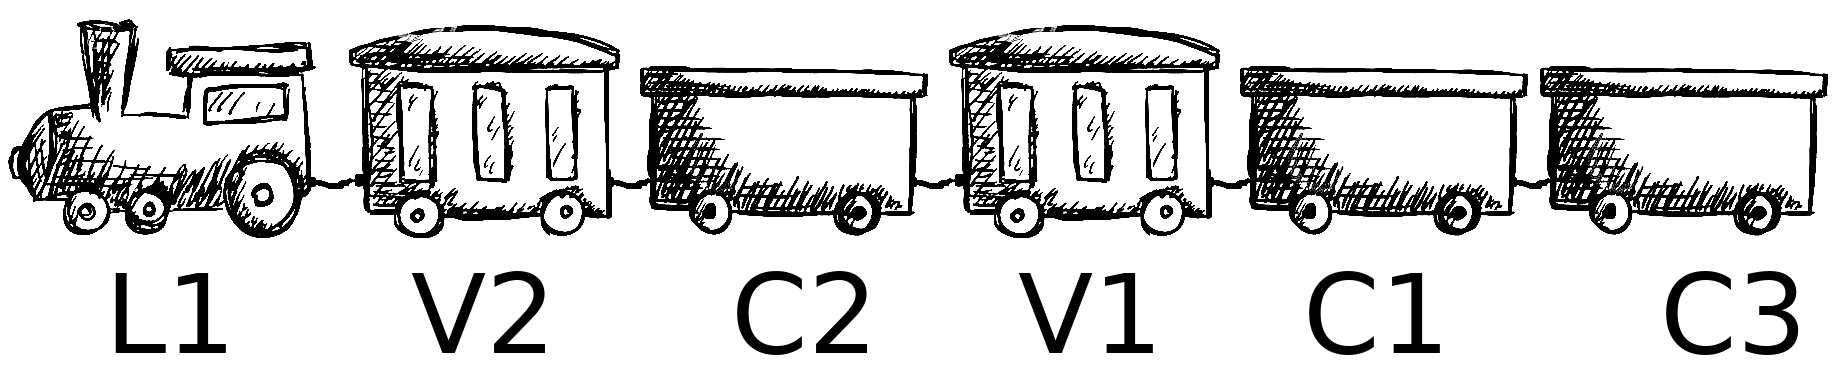
\includegraphics[width=0.8\linewidth]{MadricValencia.png}
			\end{figure}
			\begin{tabbing}
			Madr\=id-Cadiz:\\
			\>Contenedores: 3\\
			\>Vagones: 2
			\end{tabbing}
			\begin{figure}[h!]
				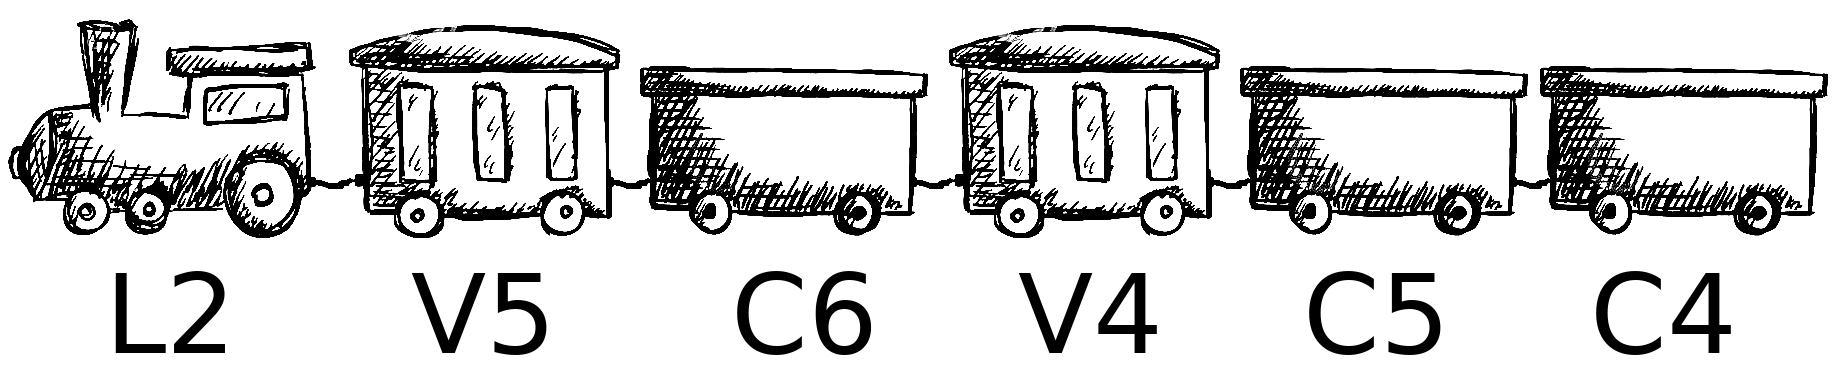
\includegraphics[width=0.8\linewidth]{MadricCadiz.png}
			\end{figure}
			\subsubsection{Mejor tipo de Vagón}
			Mirando a el cuadro \ref{tab:params1} y \ref{tab:params2rut}, se puede ver que un contenedor de 40' es objetivamente mejor ya que el coste de tranportar una tonelada por kilómetro y el precio que te cuesta una tonelada de almacenamiento al comprar los contenedores es menor en los de 40' para ambas rutas y ambas fábricas.
		\subsection{Calc frente a GLPK}
		Habiendo modelado al menos el primer trabajo en las dos plataformas, y habiendo explorando en profundidad las posibilidades que ofrece GLPK, calc es una herramienta para el modelado de tareas de programación lineal que es muy gráfico y permite ver con facilidad las restricciones, las variables y los resultados, no obstante, a diferencia de GLPK, es muy complicado hacer muchas restricciones ya que en GLPK se puede hacer de forma iterativa y en calc se tiene que poner explicitamente todas y cada una de ellas.
		
	\section{Conclusiones acerca de la práctica}
	La práctica nos ha llevado a la realización de ejercicios de programación lineal por medio de calc y de GLPK. Con ello hemos podido comprobar que el método simplex en calc puede ser beneficioso en el caso de que sea un problema muy sencillo ya que estar poniendo restricciones una a una como pasa en el caso del segundo ejercicio sería muy tedioso. Sin embargo, con GLPK se nos permite la realización de restricciones de forma iterativa lo cual puede facilitar el desarrollo del problema aunque el lenguaje empleado sea un poco complicado en un principio.\\
	También hemos conseguido entender mejor el método simplex y los tipos de funciones que se permiten en la programación lineal ya que se intentó hacer un modelo más eficiente para el modelo de la asignación pero lo más cercano que se pudo llegar a una funcion lineal con ese modelo fue usando el valor absoluto de una función, lo que no sabiamos que no era una función lineal.
	\newpage
%------------------------------------------------------------------------------------------

\end{document}